% Options for packages loaded elsewhere
\PassOptionsToPackage{unicode}{hyperref}
\PassOptionsToPackage{hyphens}{url}
\PassOptionsToPackage{dvipsnames,svgnames,x11names}{xcolor}
%
\documentclass[
]{agujournal2019}

\usepackage{amsmath,amssymb}
\usepackage{lmodern}
\usepackage{iftex}
\ifPDFTeX
  \usepackage[T1]{fontenc}
  \usepackage[utf8]{inputenc}
  \usepackage{textcomp} % provide euro and other symbols
\else % if luatex or xetex
  \usepackage{unicode-math}
  \defaultfontfeatures{Scale=MatchLowercase}
  \defaultfontfeatures[\rmfamily]{Ligatures=TeX,Scale=1}
\fi
% Use upquote if available, for straight quotes in verbatim environments
\IfFileExists{upquote.sty}{\usepackage{upquote}}{}
\IfFileExists{microtype.sty}{% use microtype if available
  \usepackage[]{microtype}
  \UseMicrotypeSet[protrusion]{basicmath} % disable protrusion for tt fonts
}{}
\makeatletter
\@ifundefined{KOMAClassName}{% if non-KOMA class
  \IfFileExists{parskip.sty}{%
    \usepackage{parskip}
  }{% else
    \setlength{\parindent}{0pt}
    \setlength{\parskip}{6pt plus 2pt minus 1pt}}
}{% if KOMA class
  \KOMAoptions{parskip=half}}
\makeatother
\usepackage{xcolor}
\setlength{\emergencystretch}{3em} % prevent overfull lines
\setcounter{secnumdepth}{5}
% Make \paragraph and \subparagraph free-standing
\ifx\paragraph\undefined\else
  \let\oldparagraph\paragraph
  \renewcommand{\paragraph}[1]{\oldparagraph{#1}\mbox{}}
\fi
\ifx\subparagraph\undefined\else
  \let\oldsubparagraph\subparagraph
  \renewcommand{\subparagraph}[1]{\oldsubparagraph{#1}\mbox{}}
\fi


\providecommand{\tightlist}{%
  \setlength{\itemsep}{0pt}\setlength{\parskip}{0pt}}\usepackage{longtable,booktabs,array}
\usepackage{calc} % for calculating minipage widths
% Correct order of tables after \paragraph or \subparagraph
\usepackage{etoolbox}
\makeatletter
\patchcmd\longtable{\par}{\if@noskipsec\mbox{}\fi\par}{}{}
\makeatother
% Allow footnotes in longtable head/foot
\IfFileExists{footnotehyper.sty}{\usepackage{footnotehyper}}{\usepackage{footnote}}
\makesavenoteenv{longtable}
\usepackage{graphicx}
\makeatletter
\def\maxwidth{\ifdim\Gin@nat@width>\linewidth\linewidth\else\Gin@nat@width\fi}
\def\maxheight{\ifdim\Gin@nat@height>\textheight\textheight\else\Gin@nat@height\fi}
\makeatother
% Scale images if necessary, so that they will not overflow the page
% margins by default, and it is still possible to overwrite the defaults
% using explicit options in \includegraphics[width, height, ...]{}
\setkeys{Gin}{width=\maxwidth,height=\maxheight,keepaspectratio}
% Set default figure placement to htbp
\makeatletter
\def\fps@figure{htbp}
\makeatother
\newlength{\cslhangindent}
\setlength{\cslhangindent}{1.5em}
\newlength{\csllabelwidth}
\setlength{\csllabelwidth}{3em}
\newlength{\cslentryspacingunit} % times entry-spacing
\setlength{\cslentryspacingunit}{\parskip}
\newenvironment{CSLReferences}[2] % #1 hanging-ident, #2 entry spacing
 {% don't indent paragraphs
  \setlength{\parindent}{0pt}
  % turn on hanging indent if param 1 is 1
  \ifodd #1
  \let\oldpar\par
  \def\par{\hangindent=\cslhangindent\oldpar}
  \fi
  % set entry spacing
  \setlength{\parskip}{#2\cslentryspacingunit}
 }%
 {}
\usepackage{calc}
\newcommand{\CSLBlock}[1]{#1\hfill\break}
\newcommand{\CSLLeftMargin}[1]{\parbox[t]{\csllabelwidth}{#1}}
\newcommand{\CSLRightInline}[1]{\parbox[t]{\linewidth - \csllabelwidth}{#1}\break}
\newcommand{\CSLIndent}[1]{\hspace{\cslhangindent}#1}

\usepackage{url} %this package should fix any errors with URLs in refs.
\usepackage{lineno}
\usepackage[inline]{trackchanges} %for better track changes. finalnew option will compile document with changes incorporated.
\usepackage{soul}
\linenumbers
\makeatletter
\makeatother
\makeatletter
\makeatother
\makeatletter
\@ifpackageloaded{caption}{}{\usepackage{caption}}
\AtBeginDocument{%
\ifdefined\contentsname
  \renewcommand*\contentsname{Table of contents}
\else
  \newcommand\contentsname{Table of contents}
\fi
\ifdefined\listfigurename
  \renewcommand*\listfigurename{List of Figures}
\else
  \newcommand\listfigurename{List of Figures}
\fi
\ifdefined\listtablename
  \renewcommand*\listtablename{List of Tables}
\else
  \newcommand\listtablename{List of Tables}
\fi
\ifdefined\figurename
  \renewcommand*\figurename{Figure}
\else
  \newcommand\figurename{Figure}
\fi
\ifdefined\tablename
  \renewcommand*\tablename{Table}
\else
  \newcommand\tablename{Table}
\fi
}
\@ifpackageloaded{float}{}{\usepackage{float}}
\floatstyle{ruled}
\@ifundefined{c@chapter}{\newfloat{codelisting}{h}{lop}}{\newfloat{codelisting}{h}{lop}[chapter]}
\floatname{codelisting}{Listing}
\newcommand*\listoflistings{\listof{codelisting}{List of Listings}}
\makeatother
\makeatletter
\@ifpackageloaded{caption}{}{\usepackage{caption}}
\@ifpackageloaded{subcaption}{}{\usepackage{subcaption}}
\makeatother
\makeatletter
\@ifpackageloaded{tcolorbox}{}{\usepackage[many]{tcolorbox}}
\makeatother
\makeatletter
\@ifundefined{shadecolor}{\definecolor{shadecolor}{rgb}{.97, .97, .97}}
\makeatother
\makeatletter
\makeatother
\ifLuaTeX
  \usepackage{selnolig}  % disable illegal ligatures
\fi
\IfFileExists{bookmark.sty}{\usepackage{bookmark}}{\usepackage{hyperref}}
\IfFileExists{xurl.sty}{\usepackage{xurl}}{} % add URL line breaks if available
\urlstyle{same} % disable monospaced font for URLs
\hypersetup{
  pdftitle={From Precipitation to Prediction: Using ConvLSTM Models for Comprehensive River Runoff Forecasting},
  pdfauthor={Florian Börgel; Sven Karsten; Karoline Rummel},
  colorlinks=true,
  linkcolor={blue},
  filecolor={Maroon},
  citecolor={Blue},
  urlcolor={Blue},
  pdfcreator={LaTeX via pandoc}}

\journalname{Climate Dynamics}

\draftfalse

\begin{document}
\title{From Precipitation to Prediction: Using ConvLSTM Models for
Comprehensive River Runoff Forecasting}

\authors{Florian Börgel\affil{1}, Sven Karsten\affil{1}, Karoline
Rummel\affil{1}}
\affiliation{1}{Leibniz-Institute for Baltic Sea Research Warnemünde, }
\correspondingauthor{Florian Börgel}{florian.boergel@io-warnemuende.de}


\begin{abstract}
a
\end{abstract}

\section*{Plain Language Summary}
b


\ifdefined\Shaded\renewenvironment{Shaded}{\begin{tcolorbox}[interior hidden, enhanced, boxrule=0pt, breakable, borderline west={3pt}{0pt}{shadecolor}, sharp corners, frame hidden]}{\end{tcolorbox}}\fi

\hypertarget{introduction}{%
\section{Introduction}\label{introduction}}

River runoff is an important component of the global water cycle as it
comprises about one third of the precipitation over land areas (Hagemann
et al., 2020). Therefore, accurate runoff forecasting is crucial for
effective water resources management, particularly over extended periods
(Fang et al., 2019; Tan et al., 2018). In the context of climate change
studies, river runoff is usually generated in two ways. First, river
runoff as input for ocean models can be created using hydrological
models such as the Hydrological Discharge (HD) model (Hagemann et al.,
2020). HD models calculate the water balance using hydrological
processes (e.g.~snow, glaciers, soil moisture, groundwater
contribution). It represents a complex forecasting tool that uses
underlying physical processes. The second approach uses data-driven
models that integrate statistical correction, using land surface schemes
of global or regional climate models {[}QUELLE{]}.

With the recent rise of machine learning in climate research various
model architectures have also been tested for river runoff forecasting.
Common approaches employ feed-forward artificial neural networks,
support vector machines, adaptive neuro-fuzzy inference systems, and
notably, Long Short-Term Memory (LSTM) neural networks that have gained
traction for long-term hydrological forecasting due to their excellent
performance (\textbf{humphrey2016hybrid?}; \textbf{huang2014monthly?};
\textbf{ashrafi2017fully?}; \textbf{liu2020streamflow?};
\textbf{fang2022application?}; \textbf{kratzert2018rainfall?}).

LSTM networks, first introduced by (\textbf{hochreiter1997long?}) , are
an evolution of the classical Recurrent Neural Networks (RNNs). Their
structure enables them to learn long-term dependencies while avoiding
the vanishing or exploding gradient problem. They have shown stability
and efficacy in sequence-to-sequence predictions. However, a limitation
of LSTMs is their inability to effectively capture two-dimensional
structures, an area where Convolutional Neural Networks (CNNs) excel.
Recognizing this limitation SHI et al. (2015) proposed a Convolutional
LSTM (ConvLSTM) architecture, which combines the strengths of both LSTM
and CNN. The ConvLSTM network has been proven useful for spatio-temporal
applications such as precipitation nowcasting (SHI et al., 2015), flood
forecasting (\textbf{moishin2021designing?}), and river runoff
forecasting (\textbf{ha2021?}; \textbf{zhu2023spatiotemporal?}).

In this work, we demonstrate that ConvLSTM networks are a reliable
method for predicting multiple rivers simultaneously, using only
atmospheric forcing, even in the absence of a fully functional
hydrological model with a complex parameterization. We use the Baltic
Sea catchment as an example to illustrate our approach. Although the
methodology we propose is universally applicable across various
geographic regions, the Baltic Sea represents a challenging region due
to its unique hydrological characteristics, being nearly decoupled from
the open ocean (see Figure). As a consequence, the salinity of the
Baltic Sea is driven to a large part by freshwater supply from rivers.
Freshwater enters the Baltic Sea through river runoff or positive net
precipitation (precipitation minus evaporation) over the sea surface.
The net precipitation accounts for 11 \(\%\) and the river input for 89
\(\%\) of the total freshwater input (\textbf{meier2002simulated?}).
Modelling the Baltic Sea is therefore to a large part the result of the
quality of the river input, that is used for the simulation. This makes
the accurate modeling of river runoff especially critical for
simulations pertaining to the Baltic Sea.

In this work we will, we present a ConvLSTM architecture that is able to
predict daily river runoff for 97 rivers across the Baltic Sea
catchment. \textbf{\emph{mehr Fokus auf Neues?}}

\hypertarget{implemented-model-architecture}{%
\section{Implemented model
architecture}\label{implemented-model-architecture}}

\hypertarget{sec-main_idea}{%
\subsection{The main idea}\label{sec-main_idea}}

We assume that the runoff at a specific point in time for all \(N_r\)
considered rivers, collected in the vector
\(\vec{R}^t \in \mathbb{R}^{N_r}\), can be accurately approximated by a
functional \(\vec{M}(\{X^t_k[x,y,\tau]\})\) of \(k=1,\ldots N_k\)
atmospheric fields \(X^t_k[x,y,\tau]\) which are known for the past
\(\tau=1,\ldots N_\tau\) time instances. This relationship is expressed
as:

\[
\begin{aligned}
\vec{R}^t = \vec{M}(\{X^t_k[x,y,\tau]\}) \ .
\end{aligned}
\]

The atmospheric fields are evaluated over a spatial domain
\(x=1,\ldots N_x\) and \(y=1,\ldots N_y\) which is sufficiently large to
capture all significant local and non-local contributions of the
atmospheric fields to the river runoff.

Typically, such a mapping is realized using a hydrological model that
simulates all relevant physical processes, transforming variables like
precipitation and evaporation into river runoff. This process relies
heavily on domain knowledge to tune all parameters to reasonable values.

As an alternative, we propose that this functional can be adequately
represented by a combination of a convolutional Long-Short Term Memory
(ConvLSTM) model with a subsequent fully connected neural network. This
approach eliminates the need for detailed knowledge of the involved
processes and their modeling. Instead, these features can be ``learned''
by the network in an automated manner. Our proposed network architecture
is visualized in Figure~\ref{fig-ConvLSTM_FC} and described in detail in
the following sections. To provide an overview, we will discuss the main
components of this architecture one-by-one.

\begin{figure}

{\centering 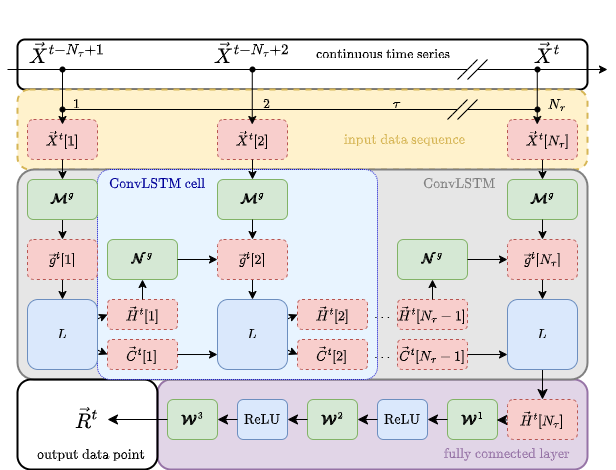
\includegraphics{./ConvLSTM_FC.png}

}

\caption{\label{fig-ConvLSTM_FC}\textbf{Combined ConvLSTM and FC network
architecture}. The starting point is the continuous timeseries of input
data \(\{\vec{X}^t\}\), upper white block. From this series, a
contiguous sequence of \(N_\tau\) elements (yellow block) is used to
feed a chain of \(N_\tau\) connected ConvLSTM cells (light blue block)
building the ConvLSTM network (grey block). The input seuqence is mapped
via weighting matrices \(\pmb{\mathcal{M}}^g\) (green blocks) onto gate
vectors \(\vec{g}^t[\tau]\). The gate vectors are then used to update
the cell state \(\vec{C}^t[\tau-1]\) and the hidden state
\(\vec{H}^t[\tau-1]\) of the last ConvLSTM cell to the current values
\(\vec{C}^t[\tau]\) and \(\vec{H}^t[\tau]\), respectively. The update is
performed with LSTM core equations collectively described by the mapping
L, see Equation~\ref{eq-LSTM}. The weighting matrices
\(\pmb{\mathcal{N}}^g\) (green blocks) control how much of the last
hidden state enters the updated state. The final output of the ConvLSTM
\(\vec{H}^t[\tau]\) is then propagated to a FC network, which itself is
a chain of three FC layers consisiting of weigthing matrices
\(\pmb{\mathcal{W}}\) and connected via ReLU functions, see
Section~\ref{sec-FC_layer}. The final result is then the river runoff
\(\vec{R}^t\) for all rivers considered at the current time instance
\(t\) (white block on the lower left). Note that all bias vectors are
ommitted for the sake of clarity. See text for more information.}

\end{figure}

\hypertarget{convlstm-network}{%
\subsection{ConvLSTM network}\label{convlstm-network}}

\hypertarget{sec-LSTM}{%
\subsubsection{The LSTM approach}\label{sec-LSTM}}

Before turning directly to the ConvLSTM the simpler architecture of the
plain Long-Short Term Memory (LSTM) model is examined which serves as a
foundation for understanding the more complex ConvLSTM.

The LSTM, a specialized form of Recurrent Neural Networks (RNNs), is
specifically designed to model temporal sequences
\(\vec{X}^t[1], \ldots \vec{X}^t[\tau],\ldots \vec{X}^t[N_\tau]\) of
\(N_\tau\) input quantities
\(\vec{X}^t[\tau] = (X^t_k[\tau]) \in \mathbb{R}^{N_k}\). This sequence
is taken from a dataset given in form of a time series \(\{\vec{X}^t\}\)
with the endpoint coinciding with the specific element in the time
series connected to time \(t\),
i.e.~\(\vec{X}^t[N_\tau] \equiv \vec{X}^t\), see
Figure~\ref{fig-ConvLSTM_FC}. Here, \(N_k\) represents the number of
input ``channels,'' which can correspond to different measurable
quantities. The LSTM's unique design allows it to adeptly handle
long-range dependencies, setting it apart from traditional RNNs in terms
of accuracy (see Figure~\ref{fig-lstm}).

\begin{figure}

{\centering 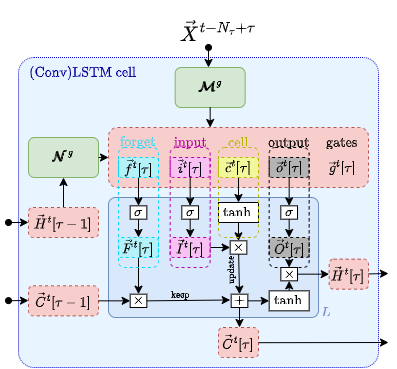
\includegraphics{./LSTM.png}

}

\caption{\label{fig-lstm}\textbf{Inner structure of a Long Short-Term
Memory Cell}. See Figure~\ref{fig-ConvLSTM_FC} and text for
information.}

\end{figure}

This performance in modeling long-range dependencies has been validated
in various studies (\textbf{XXX?}). The key component of the LSTM's
innovation is its cell state,
\(\vec{C}^t[\tau] = (C^t_h[\tau]) \in \mathbb{R}^{N_h}\), which stores
state information, also referred to as \emph{long-term memory}. This
state information complements the so-called hidden state
\(\vec{H}^t[\tau] = (H^t_h[\tau]) \in \mathbb{R}^{N_h}\) vector, which
is also known from simpler neural network architectures. In case of the
LSTM, the hidden state vector plays the role of the \emph{short-term
meory}.

A significant advantage of this architecture is the memory cell's
ability to retain gradients. This mechanism addresses the vanishing
gradient problem, where, as input sequences elongate, the influence of
initial stages becomes harder to capture, causing gradients of early
input points to approach zero. The LSTM's activation function,
inherently recurrent, mirrors the identity function with a consistent
derivative of 1.0, ensuring the gradient remains stable throughout
backpropagation.

The cell state and the hidden state are vectors, where each element is
associated with one of the \(N_h\) hidden layers, labeled by \(h\),
which are internal, \emph{artificial} degrees of freedom that enable the
high adaptibility of neural networks. These two state vectors are
determined through several self-parameterized gates, all in the same
vector space as \(\vec{C}^t[\tau]\), see Figure~\ref{fig-lstm} for a
visualization.

In particular, the forget gate \(\vec{F}^t[\tau]\) defines the portion
of the previous (long-term memory) cell state \(\vec{C}^t[\tau-1]\) that
should be kept, see dashed cyan box therein\hspace{0pt}. The input gate
\(\vec{I}^t[\tau]\) controls the contribution of the current input used
to update the long-term memory, \(\vec{C}^t[\tau]\) (magenta and yellow
boxes). The output gate, \(\vec{O}^t[\tau]\), then determines how much
of this updated long-term memory contributes to the new (short-term
memory) hidden state, \(\vec{H}^t[\tau]\) (black dashed box).

For a fixed point \(\tau\) in the sequence, the action of a LSTM cell,
i.e.~the connection between the input \(\vec{X}^t[\tau]\), the various
gates and the state vectors, is mathematically given as follows.

First, the elements of the input sequence together with the hidden state
are mapped onto auxiliary gate vectors, collectively denoted by
\(\vec{g}^t[\tau] = (g^t_h[\tau]) \in \mathbb{R}^{N_h}\), via \[
\begin{aligned}
g_h^t[\tau] =  \mathcal{M}^{g}_{hk} \, X^t_k[\tau] +  \mathcal{N}^{g}_{hh'} \, H^t_{h'}[\tau-1] + \mathcal{B}^g_{h} \ ,
\end{aligned}
\]

where \(g=i,f,o,c\) stands for the input, forget, output and cell-state
gate, respectively and Einstein's summation convention is employed,
i.e.~indices that appear twice are summed over. The calligraphic symbols
\(\mathcal{M}^{g}_{hk}, \mathcal{N}^{g}_{hh'}\) and
\(\mathcal{B}^g_{h}\) are the free parameters of the network that are
optimized for the given problem during the training, which is at the
heart of any machine learning approach. The matrix
\(\pmb{\mathcal{M}}^{g} = (\mathcal{M}^{g}_{hk}) \in \mathbb{R}^{N_h \times N_k}\)
can be interpreted as a Markovian-like contribution of the current input
\(\vec{X}^t[\tau]\) to the gates, whereas the
\(\pmb{\mathcal{N}}^{g} = (\mathcal{N}^{g}_{hh'}) \in \mathbb{R}^{N_h \times N_h}\)
scales a non-Markovian part determined by the hidden state of the last
sequence point \(\tau-1\). The vector
\(\vec{\mathcal{B}}^g = (\mathcal{B}^g_{h}) \in \mathbb{R}^{N_h}\) is a
learnable bias. It should be stressed that these parameters do neither
depend on \(t\) nor on \(\tau\) and are thus optimized once for the
complete dataset \(\{\vec{X}^t\}\).

Note that this mapping is sometimes extended by a contribution to the
\(g_h^t[\tau]\) from the past cell state \(\vec{C}^t[\tau-1]\)
(\textbf{XXX?}). Nevertheless, this mechanism called ``peeping'' is not
further considered in this work.

For the sake of brevity, we can write the mapping more compactly in
matrix-vector form as
\begin{equation}\protect\hypertarget{eq-LSTM-gates}{}{
\begin{aligned}
\vec{g}^t[\tau] = \pmb{\mathcal{M}}^{g}\vec{X}^t[\tau] + \pmb{\mathcal{N}}^{g}  \vec{H}^t[ \tau-1]+ \vec{\mathcal{B}}^g \,
\end{aligned}
}\label{eq-LSTM-gates}\end{equation}

Second, the actual gate vectors are computed by the core equations of
the LSTM as proposed by (\textbf{hochreiter1997long?}):

\begin{equation}\protect\hypertarget{eq-LSTM}{}{
\begin{aligned}
\vec{I}^t[\tau] &= \sigma(\vec{i}^t[\tau]) \\
\vec{F}^t[\tau] &= \sigma(\vec{f}^t[\tau]) \\
\vec{O}^t[\tau] &= \sigma(\vec{o}^t[\tau]) \\
\vec{C}^t[\tau] &= \vec{F}^t[\tau] \circ \vec{C}^t[\tau-1]  + \vec{I}^t[\tau] \circ \tanh(\vec{c}^t[\tau]) \\
\vec{H}^t[\tau]  &= \vec{O}^t[\tau] \circ \tanh(\vec{C}^t[\tau]) \ ,
\end{aligned}
}\label{eq-LSTM}\end{equation}

where \(\sigma\) denotes the logistic sigmoid function, \(\tanh\) is the
hyperbolic tangent and the \(\circ\) stands for the Hadamard product
(all applied in an element-wise fashion to the vectors). In the last two
equations the role of the input, forget and output gates as described
above becomes apparent.

The third step in a single layer LSTM (as employed for the work
presented here) is then to provide the output of the current LSTM cell,
i.e.~\(\vec{H}^t[\tau]\) and \(\vec{C}^t[\tau]\), to the subsequent LSTM
cell that processes the next element \(\vec{X}^t[\tau+1]\) of the input
sequence.

The full action of the LSTM network up to the end of the sequence can be
written as a nested function call

\begin{equation}\protect\hypertarget{eq-L_nested}{}{
\left(\vec{H}^t[N_\tau], \vec{C}^t[N_\tau] \right) = L \left( \vec{X}^t[N_\tau], L \left( \vec{X}^t[N_\tau-1], \ldots L \left( \vec{X}^t[1], (\vec{H}^t[0], \vec{C}^t[0]) \right) \ldots \right) \right) \ ,
}\label{eq-L_nested}\end{equation}

where
\(L\left(\vec{X}^t[\tau], \left(\vec{H}^t[\tau-1], \vec{C}^t[\tau-1] \right) \right)\)
represents Equation~\ref{eq-LSTM-gates} and Equation~\ref{eq-LSTM}. For
the present work, the initial conditions are chosen as
\(\vec{H}^t[0]=\vec{C}^t[0]=0\), which simply means that there is no
memory longer than \(N_\tau\) time steps.

The final output of the ConvLSTM chain, \(\vec{H}^t[N_\tau]\) and
\(\vec{C}^t[N_\tau]\), encode information on the full input sequence
ending at time \(t\). This information has to be decoded to obtain
useful information via an appropriate subsequent network, as it is
described in the Section~\ref{sec-FC_layer}.

\hypertarget{combining-lstm-with-spatial-convolution}{%
\subsubsection{Combining LSTM with spatial
convolution}\label{combining-lstm-with-spatial-convolution}}

Although the plain LSTM has high performance in handling temporal
sequences of point-like quantities it is not designed to recognize
spatial features in sequences of, e.g., two-dimensional maps as
atmospheric-ocean interface fields. To address this limitation we employ
a ConvLSTM architecture as described in the following.

In this kind of network the elements of the input sequence are given as
spatially varying fields
\(\vec{X}^t[\tau] = (X^t_k[x,y,\tau]) \in \mathbb{R}^{N_k \times (N_x \times N_y)}\),
where \(x\in[1, N_x]\) and \(y \in [1, N_y]\) run over the horizontal
and vertical dimensions of the map, respectively. In order to enable the
``learning'' of spatial patterns, the free parameters of the network are
replaced by two-dimensional convolution kernels
\(\pmb{\mathcal{M}}^{g} = (\mathcal{M}^{g}_{hk}[\xi, \eta]) \in \mathbb{R}^{(N_h \times N_k)\times (N_\xi \times N_\eta)}\)
and
\(\pmb{\mathcal{N}}^{g} = (\mathcal{N}^{g}_{hh'}[\xi, \eta]) \in \mathbb{R}^{(N_h \times N_h)\times (N_\xi \times N_\eta)}\).
The width and the height of the kernels are given by \(N_\xi\) and
\(N_\eta\), respectively and
\(\xi\in [-(N_\xi-1)/2,(N_\xi-1)/2], \eta\in [-(N_\eta-1)/2,(N_\eta-1)/2]\),
where, without loss of generality, we assume odd numbers for the kernel
sizes.

The mapping from the input quantities to the gates is then given by a
convolution with these kernels \[
\begin{aligned}
g^t_h[x,y,\tau] & =  \mathcal{M}^{g}_{hk} [\xi,\eta]\, X^t_k[x-\xi, y-\eta, \tau]  +  \mathcal{N}^{g}_{hh'}[\xi,\eta] \, H^t_{h'}[x-\xi, y-\eta, \tau-1] + \mathcal{B}^g_{h}\ .
\end{aligned}
\]

again with Einstein's convention imposed.

It becomes immediately apparent that in case of the ConvLSTM, the gate
and state vectors must become vector fields
(\(\in \mathbb{R}^{N_h \times (N_x \times N_y)}\)) as well. We can write
this mapping in the same way as Equation~\ref{eq-LSTM-gates} but with
replacing the normal matrix-vector multiplication by a convolution
(denoted with \(\ast\)), i.e.\\
\[
\begin{aligned}
\vec{g}^t[\tau] = \pmb{\mathcal{M}}^{g} \ast \vec{X}^t[\tau] + \pmb{\mathcal{N}}^{g} \ast  \vec{H}^t[ \tau-1]+ \vec{\mathcal{B}}^g \,
\end{aligned}
\]

The subsequent processing of the \(\vec{g}^t[\tau]\) remains
symbolically the same as presented in Equation~\ref{eq-LSTM} but with
all appearing quantities now meaning vector fields instead of simple
vectors.

In summary, the ConvLSTM excels at processing tasks that demand a
combined understanding of spatial patterns and temporal sequences in
data. It merges the image-processing capabilities of Convolutional
Neural Networks (CNNs) with the time-series modeling of Long Short-Term
Memory (LSTM) networks.

\hypertarget{sec-FC_layer}{%
\subsection{Fully connected layer}\label{sec-FC_layer}}

As stated in Sec. Section~\ref{sec-LSTM}, the final output
\(\vec{H}^t[N_\tau]\) and \(\vec{C}^t[N_\tau]\) of the ConvLSTM encode
information on the full input sequence. In order to contract this
information to obtain the runoff vector \(\vec{R}^t\) representing the
\(N_r\) rivers, we propose to subject the final short-term memory
(i.e.~the hidden state \(\vec{H}^t[N_\tau]\)) to an additional FC
network.

In particular, the dimensionality of the vector field
\(\vec{H}^t[N_\tau]\) is sequentially reduced by three nested FC layers,
each connected to the other by the Rectified Linear Unit (ReLU), see
Figure~\ref{fig-ConvLSTM_FC}. Integrating over artificial degrees of
freedom in a step-wise fashion has turned out to be benificial
{[}(\textbf{XXX?}){]}.

Spelled out in mathematics, the runoff of the \(r\)-th river is then
obtained via (using Einstein's convention)

\[
\begin{aligned}
R_r^t = \mathcal{W}^{3}_{rb}\mathrm{ReLU}\left(\mathcal{W}^{2}_{ba}\mathrm{ReLU}\left(\mathcal{W}^{1}_{ah} [x,y] H^t_h[x,y, N_\tau] + \mathcal{B}^1_a\right) + \mathcal{B}^2_b \right) + \mathcal{B}^3_r \ ,
\end{aligned}
\]

where \(a=1,\ldots N_a\), \(b=1,\ldots N_b\) and the hyper parameters
\(N_a\) and \(N_b\) are chosen such that
\(N_h\cdot N_x\cdot N_y > N_a > N_b > N_r\) in order to achieve the
aforementioned step-by-step reduction of dimensionality. The weights
\(\mathcal{W}\) and biases \(\mathcal{B}\) stand for parameters that are
optimized during the training of the network.

In matrix-vector notation this can be compactified to \[
\begin{aligned}
\vec{R}^t = \pmb{\mathcal{W}}^{3}\mathrm{ReLU}\left(\pmb{\mathcal{W}}^{2}\mathrm{ReLU}\left(\pmb{\mathcal{W}}^{1} \vec{H}^t[N_\tau] + \vec{\mathcal{B}}^1\right) + \vec{\mathcal{B}}^2 \right) + \vec{\mathcal{B}}^3 \ .
\end{aligned}
\]

Combining the last equation with Equation~\ref{eq-L_nested} provides
finally an explicit formula for the initial assumption of modelling the
runoff for time \(t\) as a functional of a sequence of atmospheric
fields, i.e.

\[
\begin{aligned}
\vec{R}^t & = \vec{M}(\{X^t_k[x,y,\tau]\}) \\
& = \pmb{\mathcal{W}}^{3}\mathrm{ReLU}\left(\pmb{\mathcal{W}}^{2}\mathrm{ReLU}\left(\pmb{\mathcal{W}}^{1} \vec{L}_H \left( \vec{X}^t[N_\tau], L \left( \vec{X}^t[N_\tau-1], \ldots L \left( \vec{X}^t[1], (0, 0) \right) \ldots \right) \right) + \vec{\mathcal{B}}^1\right) + \vec{\mathcal{B}}^2 \right) + \vec{\mathcal{B}}^3 \ ,
\end{aligned}
\] where the \(\vec{L}_H\) means that only the hidden state vector of
the final ConvLSTM call is forwarded to the FC layer.

In Section~\ref{sec-technical_details}, we present the employed model
and data setup as well as the choice for all mentioned hyper parameters
that lead to an adequate model performance after training.

\hypertarget{sec-technical_details}{%
\section{Technical details}\label{sec-technical_details}}

\hypertarget{runoff-data-used-for-training}{%
\subsection{Runoff data used for
training}\label{runoff-data-used-for-training}}

The runoff data covering the period 1979 to 2011 is based on an E-HYPE
hindcast simulation that was forced by a regional downscaling of
ERA-Interim (\textbf{dee2011?}) with RCA3 (\textbf{theross?}) and
implemented into NEMO-Nordic (\textbf{hordoir2019?}) as a mass flux. For
the periods before (1961 to 1978) and after (2012 to 2018) additional
spatial temporal corrections have been applied to the runoff data, and
have therefore been ignored. The quality of the runoff was extensively
evaluated. For more information see (\textbf{gröger2022?}) and
references therein.

\hypertarget{atmospheric-forcing}{%
\subsection{Atmospheric Forcing}\label{atmospheric-forcing}}

The UERRA-HARMONIE regional reanalysis dataset was developed as part of
the FP7 UERRA project (Uncertainties in Ensembles of Regional
Re-Analyses, \href{http://www.uerra.eu/}{http://www.uerra.eu/)},). The
UERRA-HARMONIE system represents a comprehensive, high-resolution
reanalysis covering a wide range of essential climate variables. This
dataset encompasses data on air temperature, pressure, humidity, wind
speed and direction, cloud cover, precipitation, albedo, surface heat
fluxes, and radiation fluxes from January 1961 to July 2019. With a
horizontal resolution of 11 km and analyses conducted at 00 UTC, 06 UTC,
12 UTC, and 18 UTC, it also provides hourly resolution forecast model
data. UERRA-HARMONIE is accessible through the Copernicus Climate Data
Store (CDS, \url{https://cds.climate.copernicus.eu/\#!/home),} initially
produced during the UERRA project and later transitioned to the
Copernicus Climate Change Service (C3S,
\url{https://climate.copernicus.eu/copernicus-regionalreanalysis-europe).}

\hypertarget{ocean-model}{%
\subsection{Ocean Model}\label{ocean-model}}

To simulate the Baltic Sea, we use a coupled 3-dimensional ocean model
Baltic Sea, called the Modular Ocean Model (MOM). This model uses a
finite-difference method to solve the full set of primitive equations to
calculate the motion of water and the transport of heat and salt. The
K-profile parameterization (KPP) was used as turbulence closure scheme.
The model's western boundary opens into the Skagerrak and connects the
Baltic Sea to the North Sea. The maximum depth was set at 264 meters. A
more detailed description of the setup can be found in
(\textbf{gröger2022?}).

\hypertarget{neural-network-hyper-parameters}{%
\subsection{Neural network hyper
parameters}\label{neural-network-hyper-parameters}}

\begin{figure}

{\centering \includegraphics{ConvLSTM.png}

}

\caption{\label{fig-baltNet}Schematic structure of the ConvLSTM
implementation for river runoff forecasting.}

\end{figure}

For the computation we use the following set of hyper parameters:

\hypertarget{tbl-letters}{}
\begin{longtable}[]{@{}ll@{}}
\caption{\label{tbl-letters}Hyperparameters}\tabularnewline
\toprule()
Parameter name & Parameter size \\
\midrule()
\endfirsthead
\toprule()
Parameter name & Parameter size \\
\midrule()
\endhead
Channel size & 4 \\
Num. hidden layer & 9 \\
Num. timesteps & 30 \\
Conv. Kernelsize & (7,7) \\
Num. ConvLSTM layers & 1 \\
Batch size & 50 \\
Learning Rate & 1e-3 with CosineAnnealing \\
\bottomrule()
\end{longtable}

As input the model receives \(N_{\tau}\) = 30 days of atmospheric
surface fields temperature \(T\), precipitation \(P\), specific humidity
\(Q\) and wind speed \(W\), with a daily resolution to predict the river
runoff \(\vec{R}\). The choice of atmospheric fields was based on the
implemented river runoff calculation in the atmospheric model COSMO-CLM
which uses these atmospheric fields to calculate an river runoff
estimate.

\hypertarget{results}{%
\section{Results}\label{results}}

The model was trained with daily data for the period 1979 to 2011, as
this period represents the only period of E-HYPE without further bias
correction applied to the runoff to match observations. The data was
divided into randomly chosen splits of 80\(\%\) training data, 10\(\%\)
validation data to evaluate the performance of the model during
training, and 10\(\%\) training data which is finally used to evaluate
the performance of the model after training. The model was trained for
400 epochs and the model weights with the lowest mean squared error
during training have been stored.

The accuracy of the model is displayed in Figure
\textbf{?@fig-statistical-evaluationNN}. As mention above for
evaluation, the test dataset was utilized. The left panel panel (Figure
\textbf{?@fig-statistical-evaluationNN} a) illustrates the relative
prediction error in relation to the original E-HYPE data, indicating
that, on daily timescales, the model can predict river runoff with an
accuracy of \(\pm\) 5\(\%\). The overall correlation is 0.997 with the
resulting error metrics yielding a RMSE of 323.99 \(m^3\)/s and MAE of
249.51 \(m^3\)/s. While the model's performance is satisfactory, the
discrepancies between the actual values and the predictions could partly
be attributed to the use of a different atmospheric dataset than the one
originally used to drive the E-HYPE model. However, by applying a
rolling mean with a 5-day window, the prediction error is reduced to
less than 1\(\%\), which is acceptable for the purposes of climate
modeling. Lastly, the right panel demonstrates that the distribution of
residuals follows a Gaussian shape, suggesting that our model does not
exhibit bias by systematically over or underestimating river runoff
values.

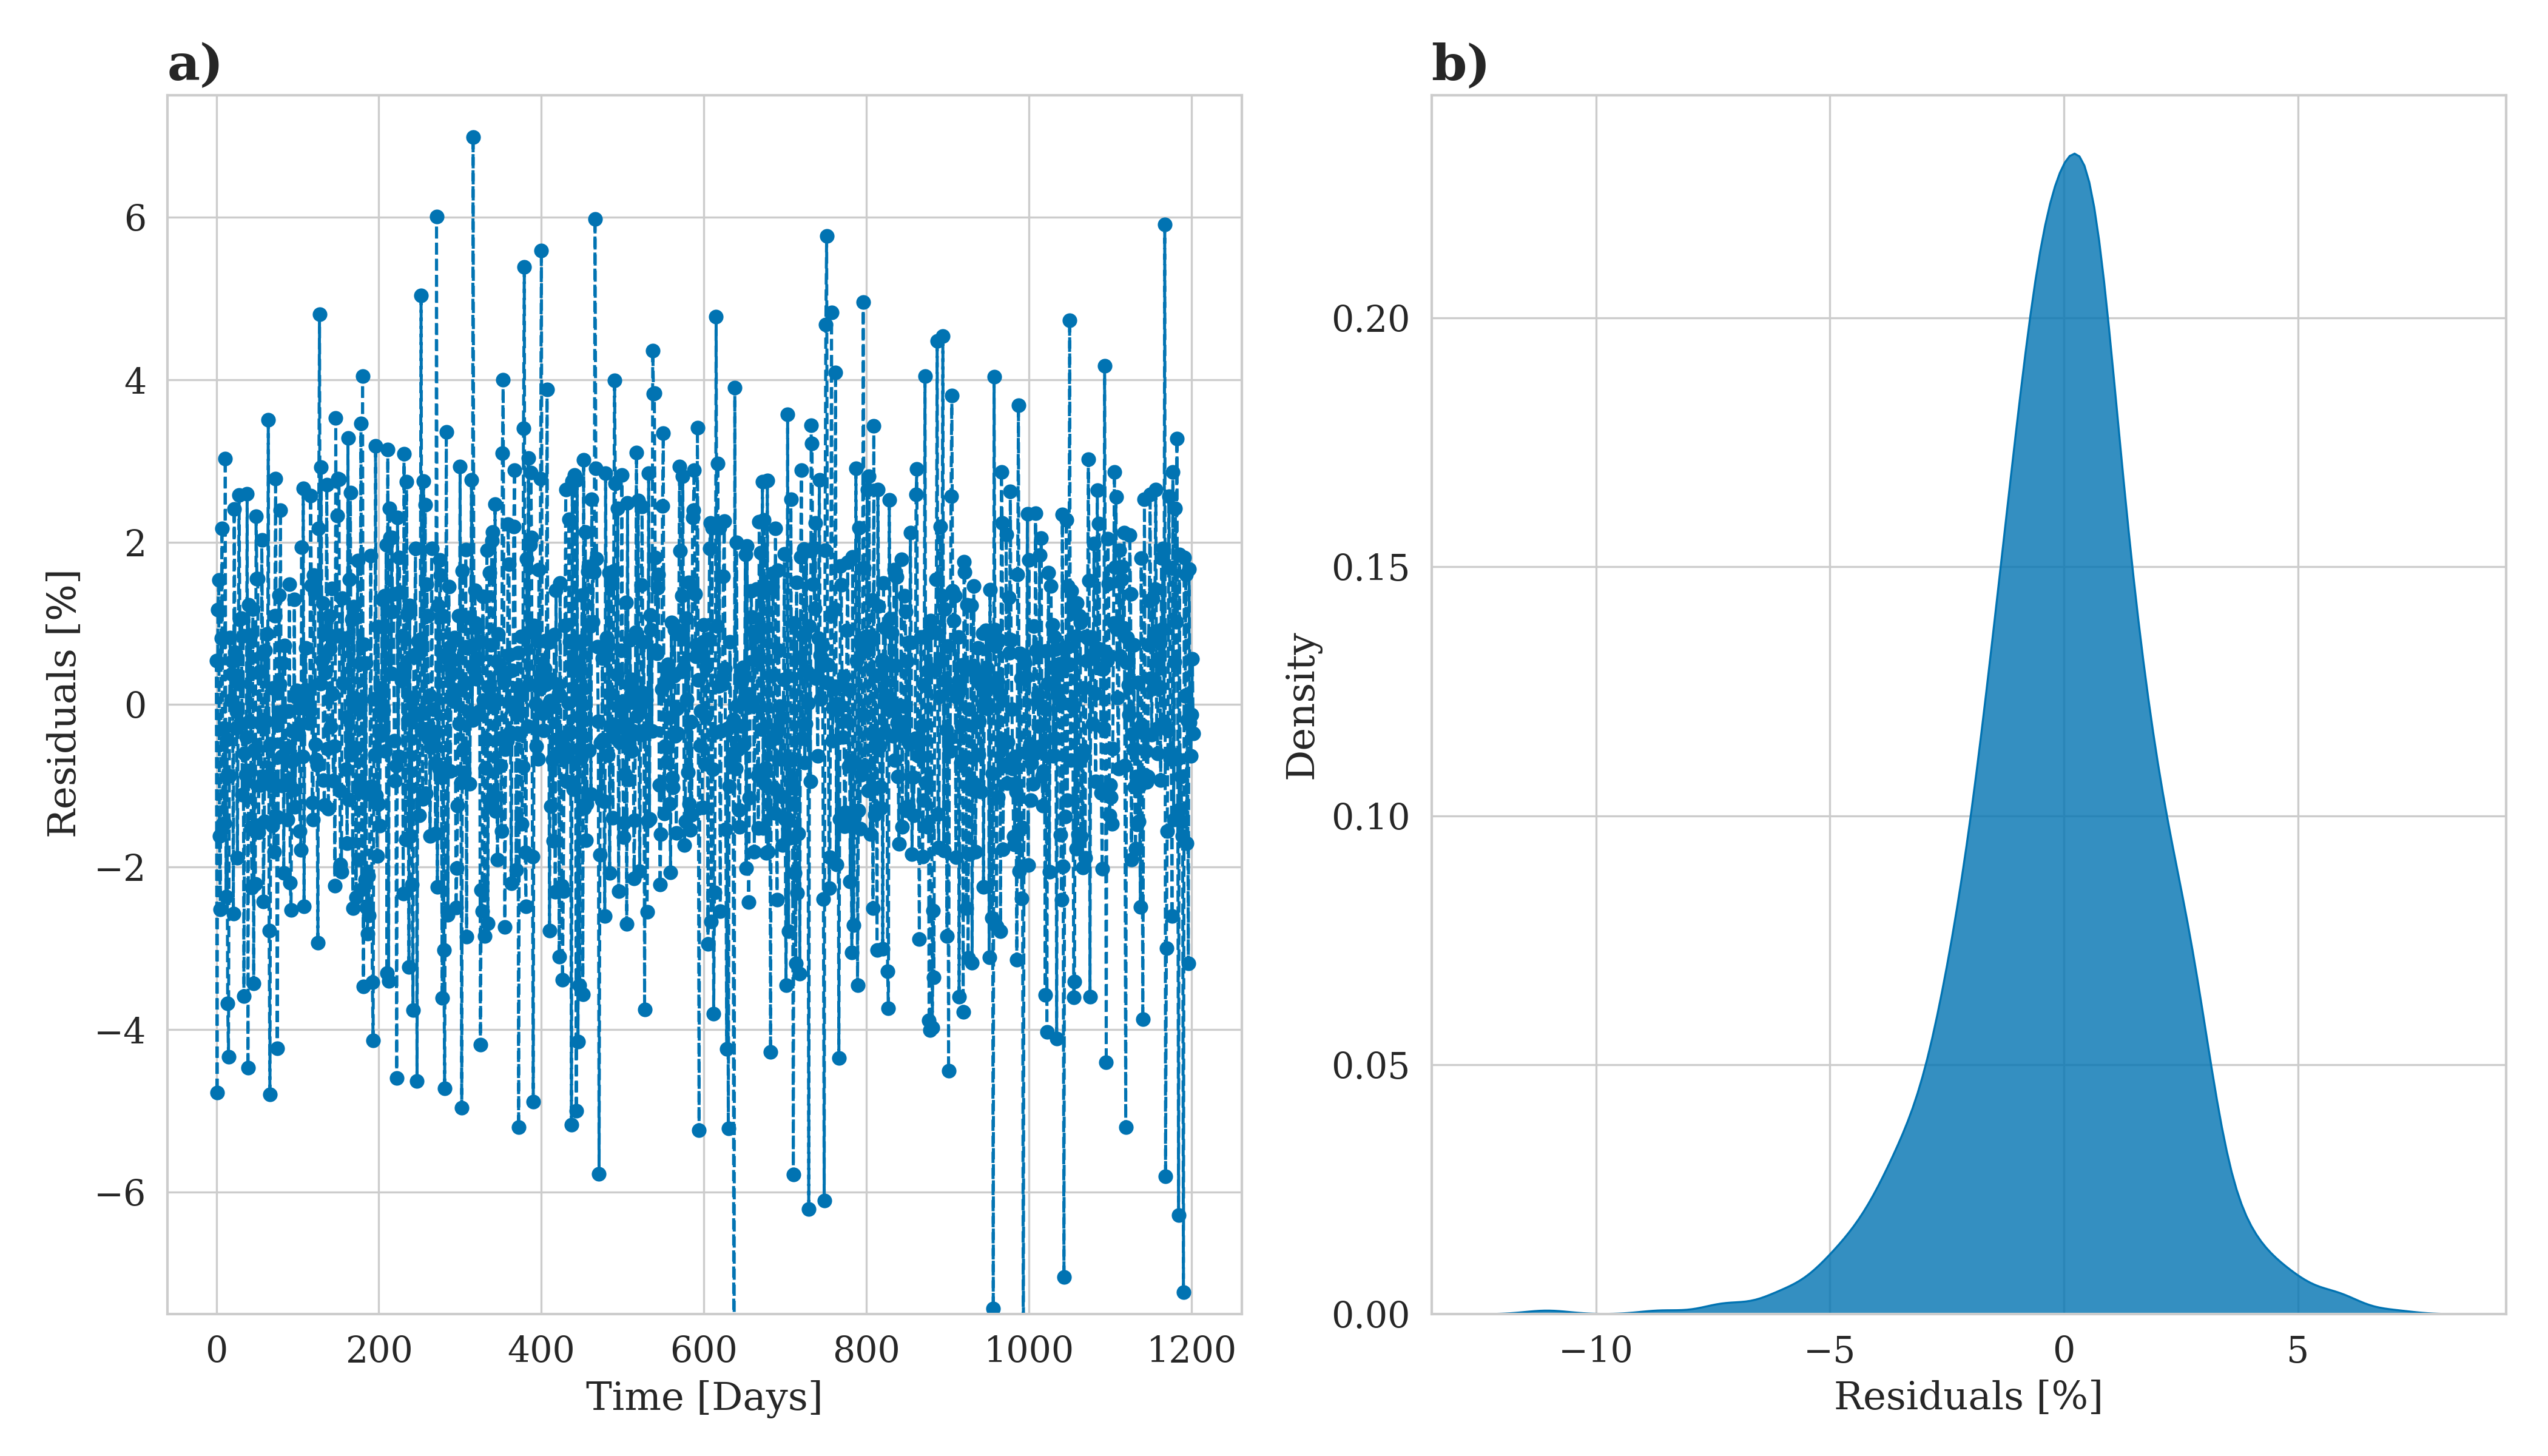
\includegraphics{../src/figures/paper_error_metrics.png}

In the following we will now address the overall performance of the
total river runoff while also zooming in on the four largest rivers
entering the Baltic Sea. @fig-PerformanceNeuralNetworkRunoff shows the
predicted and the original river runoff using the test dataset. The
predicted total river runoff for the Baltic Sea is closely matching the
original data (@fig-PerformanceNeuralNetworkRunoff a). Zooming in on the
largest individual rivers (@fig-PerformanceNeuralNetworkRunoff b-e) it
can be seen that that also the prediction of the individual rivers is
close to the original data.

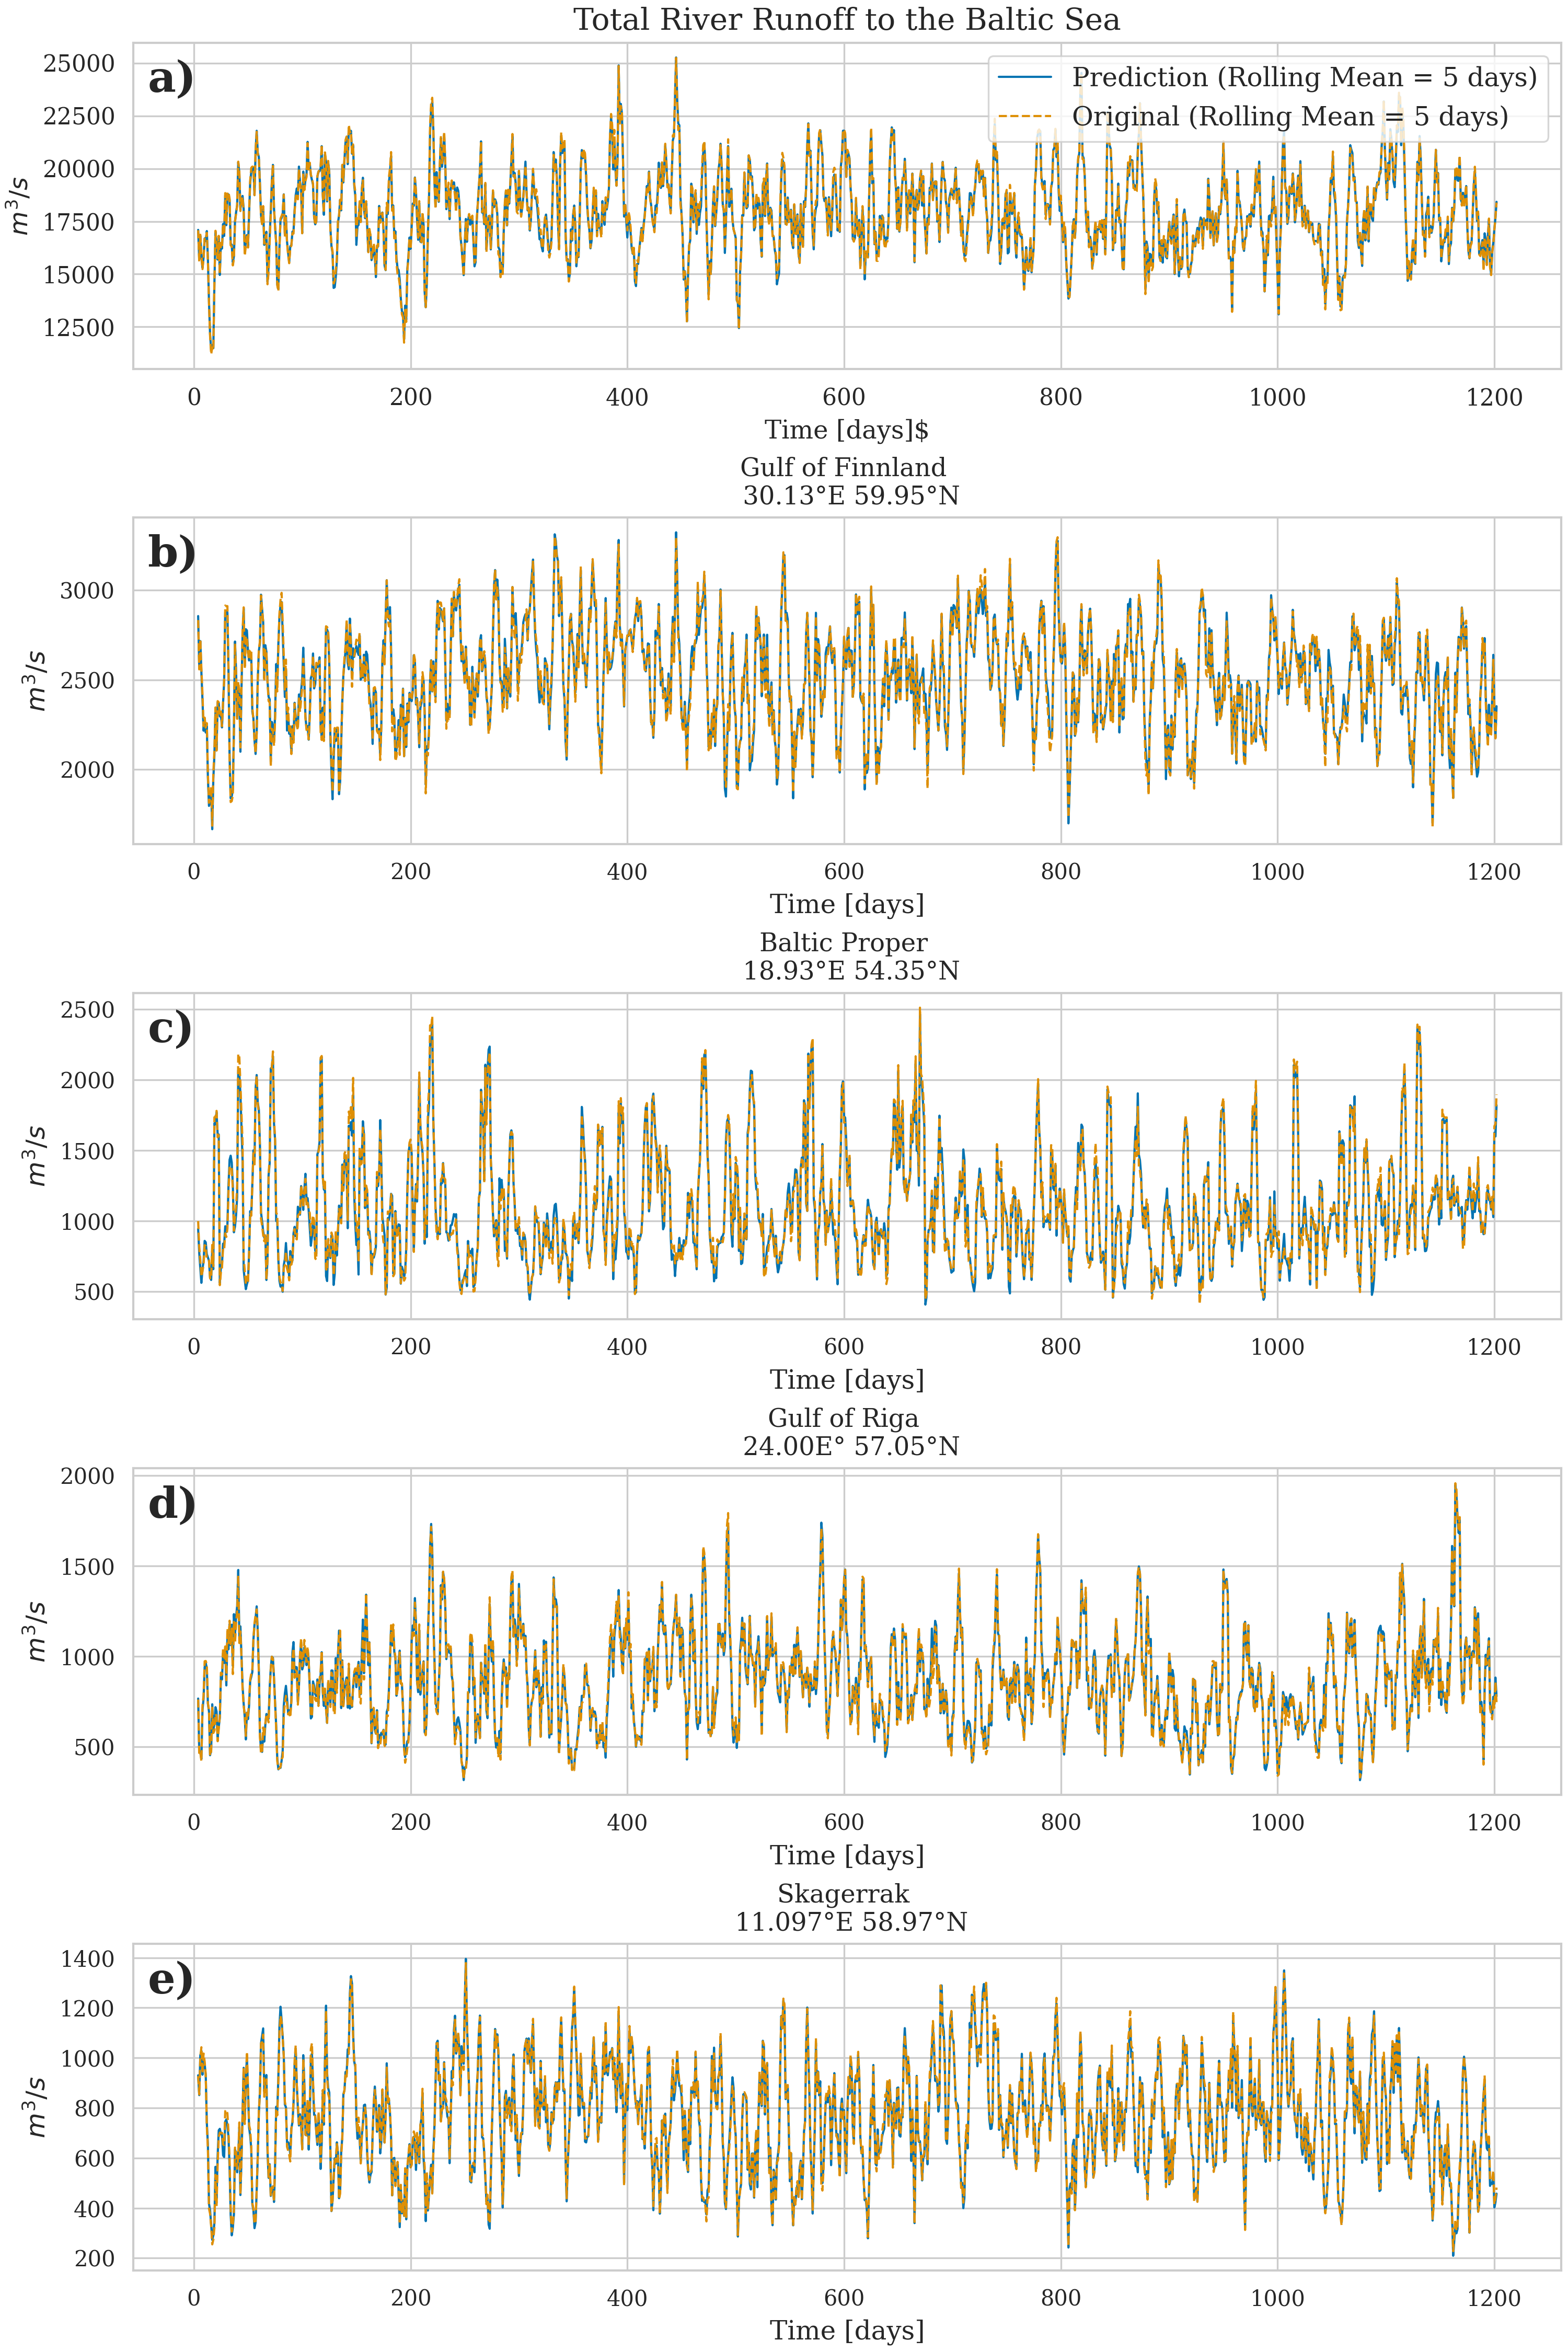
\includegraphics{../src/figures/paper_total_river_runoff.png}

Lastly, we evaluated the performance of the runoff model by
incorporating the predicted river runoff as runoff forcing into the
ocean model MOM5. This provides a robust validation of the runoff model
against more complex real world conditions. This allows us to ensure
that the predictions accurately reflect the impact of the river
discharge on the ocean dynamics, validating the temporal and spatial
variability of the the river discharge. \textbf{?@fig-by15} shows the
salinity comparison between the original E-HYPE river runoff and the
predicted river runoff at BY15 - a central stations in the Baltic Sea.
It can be seen that the model simulation using the predicted river
runoff by the ConvLSTM is closely mirroring the control simulation. The
upper panel (\textbf{?@fig-by15} a) shows the surface salinity,
representing the high-frequency variations in the salinity, which is
heavily affected by river runoff. The lower panel (\textbf{?@fig-by15}
b) shows the bottom salinity which can be viewed as a low-pass filter in
the Baltic Sea, which is also closely mirrored by the ConvLSTM
predictions.

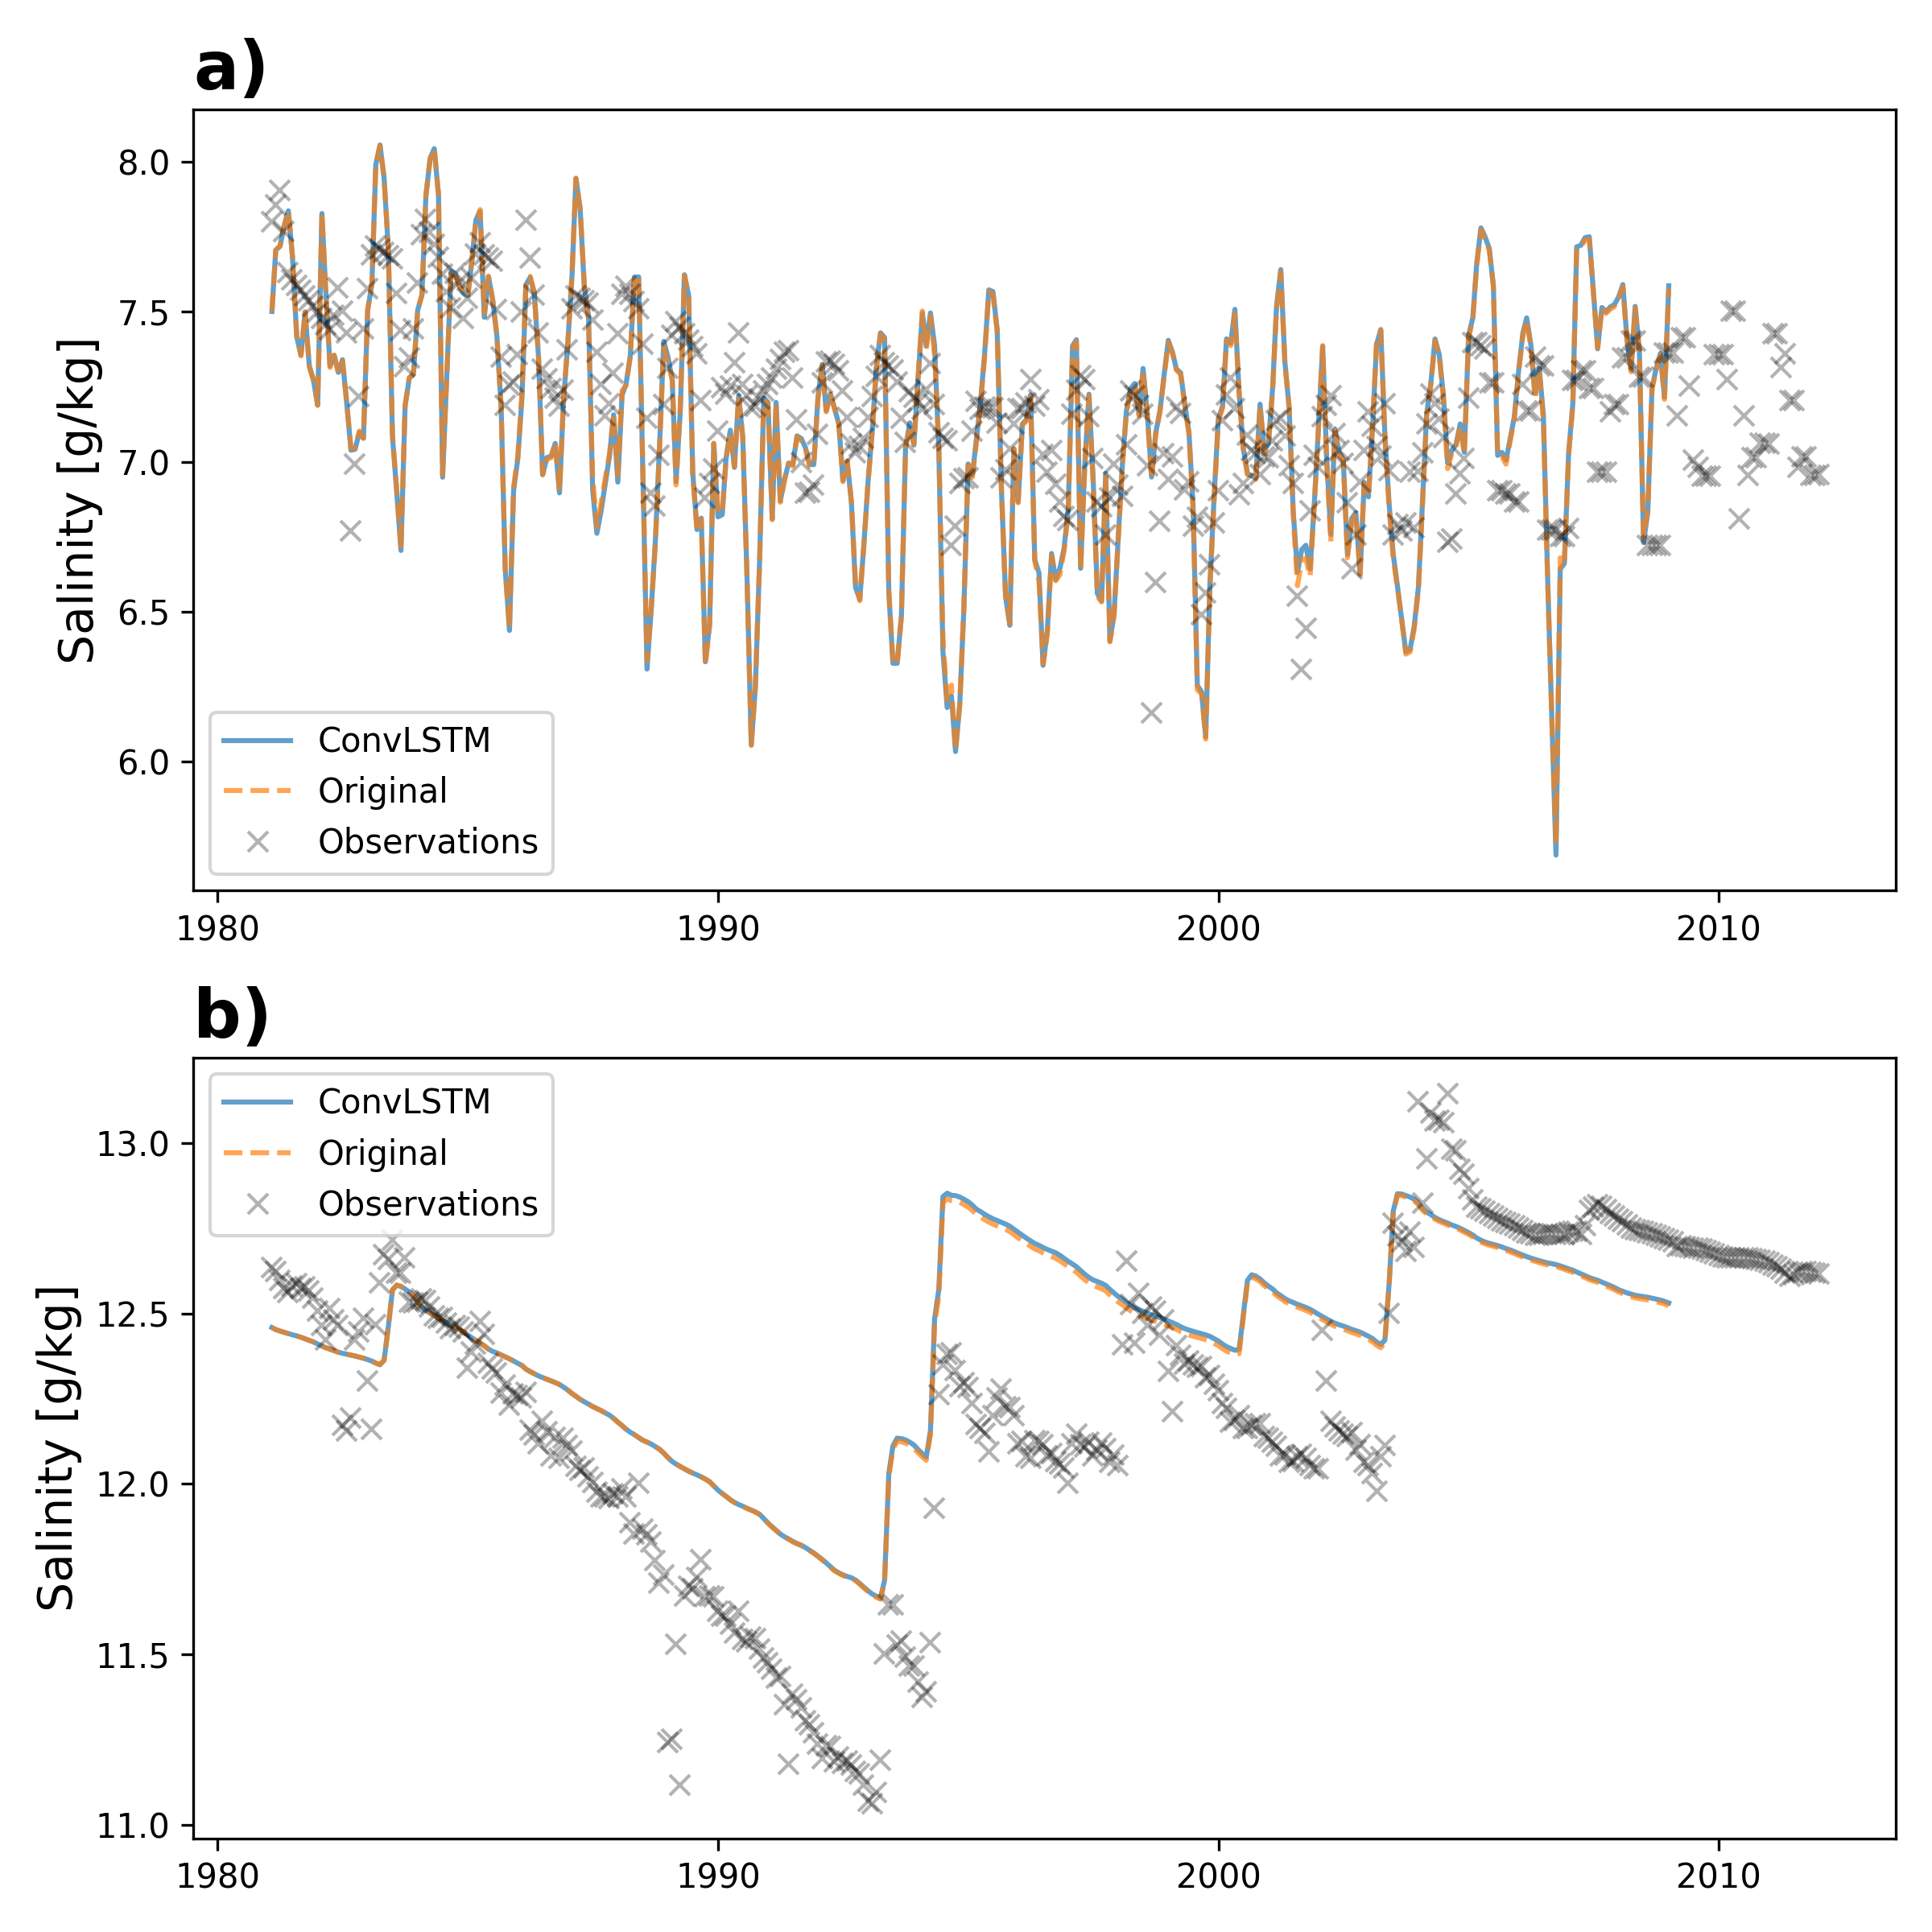
\includegraphics{../src/figures/by15_model.png}

The final evaluation of the ConvLSTM model concentrates on the spatial
accuracy of river runoff predictions. Figure xxx a) shows the vertically
averaged salinity for the period 1981 to 2011 in the reference
simulation. It highlights the strong horizontal gradients and complex
topographic features in the Baltic Sea, as evidenced by salinity
variations in deeper waters, captured by the vertical integration.
Figure 4b compares these results by showing the percentage difference in
vertically averaged salinity between the ConvLSTM simulation and the
reference simulation. Overall, the differences remain below 1\(\%\),
except near a river mouth in the Gulf of Riga (22-24°E, 56.5-58.5°N for
orientation), where the difference is approximately 1\(\%\).

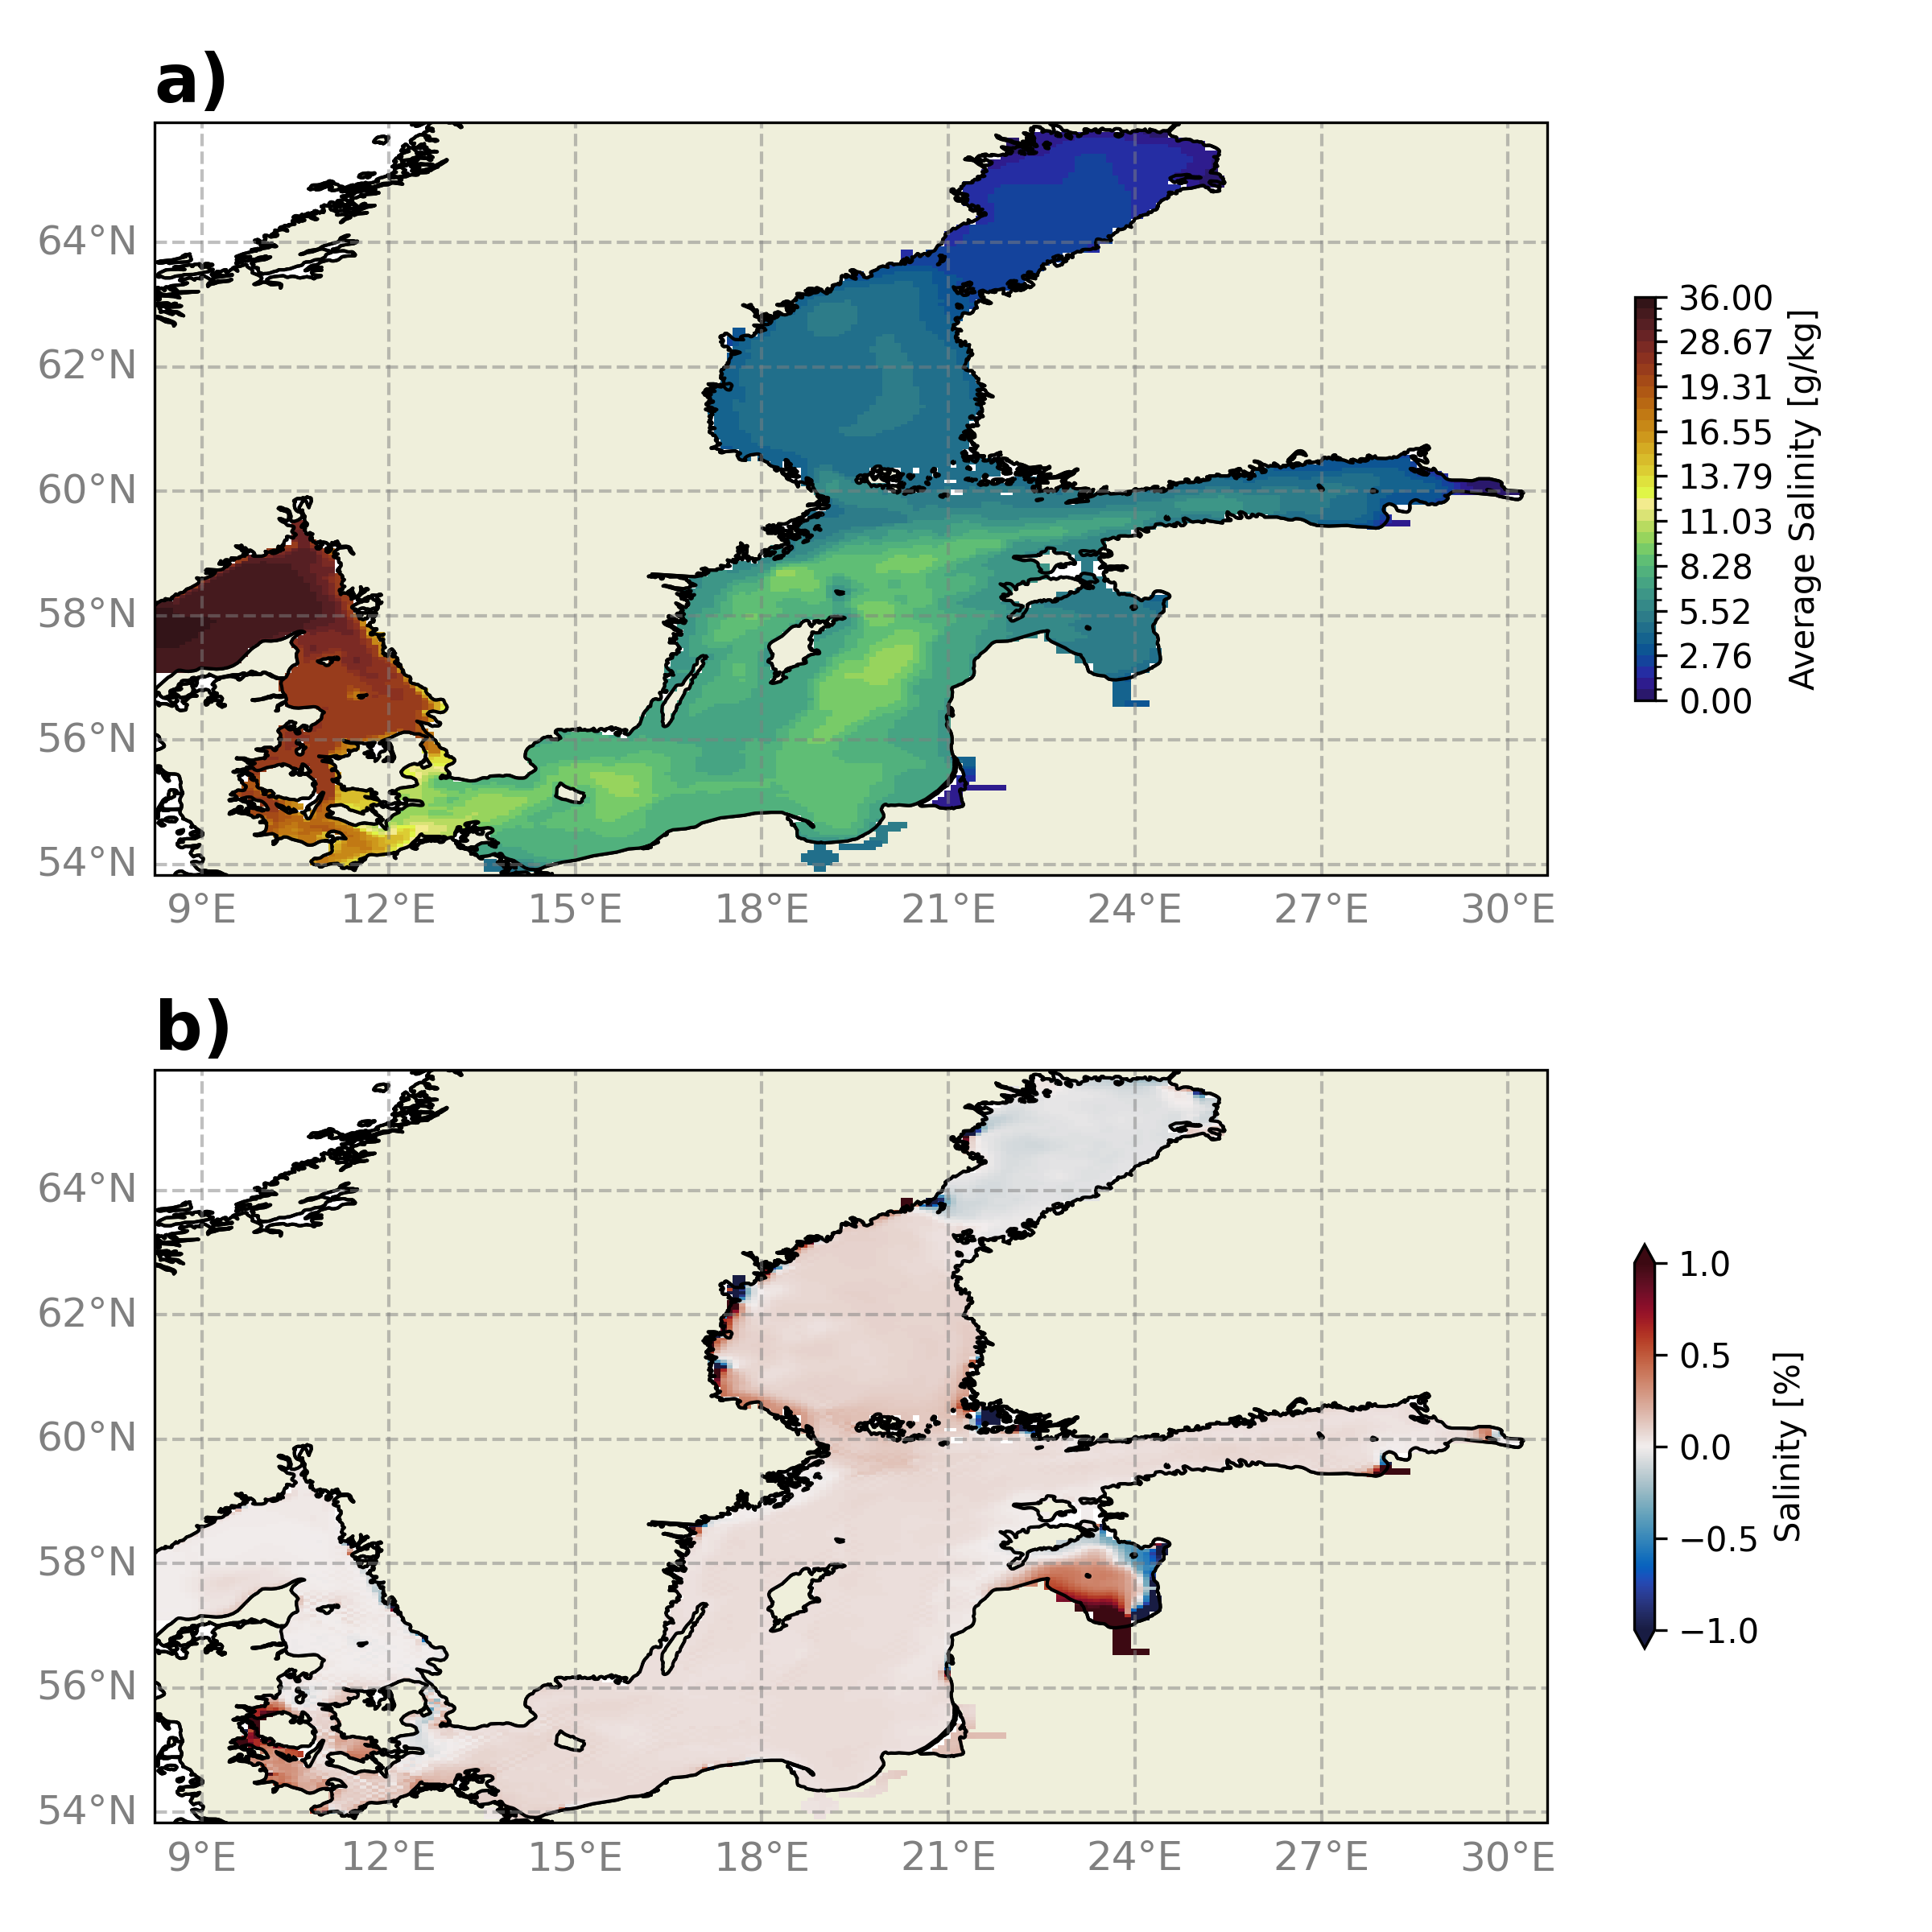
\includegraphics{../src/figures/evaluation_MOM.png}

\hypertarget{discussion}{%
\section{Discussion}\label{discussion}}

With the increasing demand of decision makers for regional climate
projections, that allow to quantify regional climate change impacts, the
availability of precise hydrological forecasting becomes invaluable. The
quality of a projection for a coastal sea such as the Baltic Sea is too
large parts based on the quality of the hyrdological conditions. In this
work we analyze the implementation of a ConvLSTM networks for predicting
river runoff, highlighting its potential to enhance river runoff
forecasting across different coastal seas. Given the unique hydrological
characteristics of the Baltic Sea, largely influenced by its limited
connection to the open ocean and significant freshwater input from
surrounding rivers, the region presents a critical case for the
application of sophisticated forecasting models.

The transition from traditional hydrological models to machine learning
approaches, such as the ConvLSTM model, offers significant advantages.
The ConvLSTM can be seamlessly integrated into regional climate models,
allowing for the real-time computation of river runoff while performing
climate projections. While the initial training of the model requires
substantial computational resources, it remains less intensive than
running comprehensive hydrological models. Furthermore, once trained,
the ConvLSTM model is computationally efficient during inference,
ensuring enhanced forecasting capabilities without significantly
increasing computational demands.

While the ConvLSTM represents an advancement for the climate community,
given that running and tuning traditional hydrological models demands
extensive expertise, models like E-HYPE maintain an essential role. They
provide a comprehensive dataset that helps to train our ConvLSTM model
effectively. This robust training enables the machine learning models to
achieve highly accurate predictive weights. Thus, rather than rendering
traditional methods obsolete, the integration of machine learning models
builds upon and enhances the foundational data provided by them.

The robust performance of the ConvLSTM model in simulating river runoff
and its possible effective integration into regional climate models pave
the way for a multitude of new storyline simulations. Hence, we can now
explore various ``what-if'' scenarios more reliably, under the
assumption that the model weights attained during training are robust.

In summary, we showed that the ConvLSTM model demonstrated robust
performance in forecasting river runoff across 97 rivers entering the
Baltic Sea. Trained on data from 1979 to 2011, the model achieved an
impressive daily prediction accuracy of ±5\(\%\). This capability to
generate accurate and detailed simulations enables to examine the
potential impacts of different climate scenarios. Such precision in
forecasting and scenario testing is crucial for crafting effective water
resource management strategies and adapting to the changing climate.

Ultimately, the integration of ConvLSTM into regional climate models
represents a significant step forward in our ability to understand and
predict the complex dynamics of river systems and their impact on
regional climate systems.

\hypertarget{acknowledgments}{%
\section{Acknowledgments}\label{acknowledgments}}

The research presented in this study is part of the Baltic Earth program
(Earth System Science for the Baltic Sea region, see
\href{https://www.baltic.earth/}{https://www.baltic.earth}.

\hypertarget{references}{%
\section*{References}\label{references}}
\addcontentsline{toc}{section}{References}

\hypertarget{refs}{}
\begin{CSLReferences}{1}{0}
\vspace{1em}

\leavevmode\vadjust pre{\hypertarget{ref-fangExaminingApplicabilityDifferent2019}{}}%
Fang, W., Huang, S., Ren, K., Huang, Q., Huang, G., Cheng, G., \& Li, K.
(2019). Examining the applicability of different sampling techniques in
the development of decomposition-based streamflow forecasting models.
\emph{Journal of Hydrology}, \emph{568}, 534--550.
\url{https://doi.org/10.1016/j.jhydrol.2018.11.020}

\leavevmode\vadjust pre{\hypertarget{ref-hagemannHighResolutionDischarge2020}{}}%
Hagemann, S., Stacke, T., \& Ho-Hagemann, H. T. M. (2020). High
{Resolution Discharge Simulations Over Europe} and the {Baltic Sea
Catchment}. \emph{Frontiers in Earth Science}, \emph{8}.
\url{https://doi.org/10.3389/feart.2020.00012}

\leavevmode\vadjust pre{\hypertarget{ref-shiConvolutionalLSTMNetwork2015}{}}%
SHI, X., Chen, Z., Wang, H., Yeung, D.-Y., Wong, W., \& WOO, W. (2015).
Convolutional {LSTM Network}: {A Machine Learning Approach} for
{Precipitation Nowcasting}. In \emph{Advances in {Neural Information
Processing Systems}} (Vol. 28). Curran Associates, Inc. Retrieved from
\url{https://proceedings.neurips.cc/paper/2015/hash/07563a3fe3bbe7e3ba84431ad9d055af-Abstract.html}

\leavevmode\vadjust pre{\hypertarget{ref-tanAdaptiveMiddleLongterm2018}{}}%
Tan, Q.-F., Lei, X.-H., Wang, X., Wang, H., Wen, X., Ji, Y., \& Kang,
A.-Q. (2018). An adaptive middle and long-term runoff forecast model
using {EEMD-ANN} hybrid approach. \emph{Journal of Hydrology},
\emph{567}, 767--780.
\url{https://doi.org/10.1016/j.jhydrol.2018.01.015}

\end{CSLReferences}



\end{document}
